	\chapter{Planificación y Gestión del Proyecto}

	\section{Metodología}
	Se utiliz\'o la metodolog\'ia SCRUM, ya que con esta se tienen todos los requerimientos a la mano, donde cada \textit{issue} tiene que ser definido detalladamente, sea una tarea, una historia de usuario, o un bug. Esta metodolog\'ia ata los \textit{issues} a un bloque de tiempo determinado llamado \textit{sprint}, donde as\'i, las fechas de entrega pueden definirse de una manera m\'as clara, y el manejo del tiempo de los desarrolladores es gestionado de mejor manera.
	\section{Fuentes}
	\begin{itemize}
		\item Repositorio Backend de GitHub
		\item Repositorio Frontend de GitHub
		\item JIRA
	\end{itemize}

	\section{Cronograma}
	\begin{figure}[h!]
		\centering
		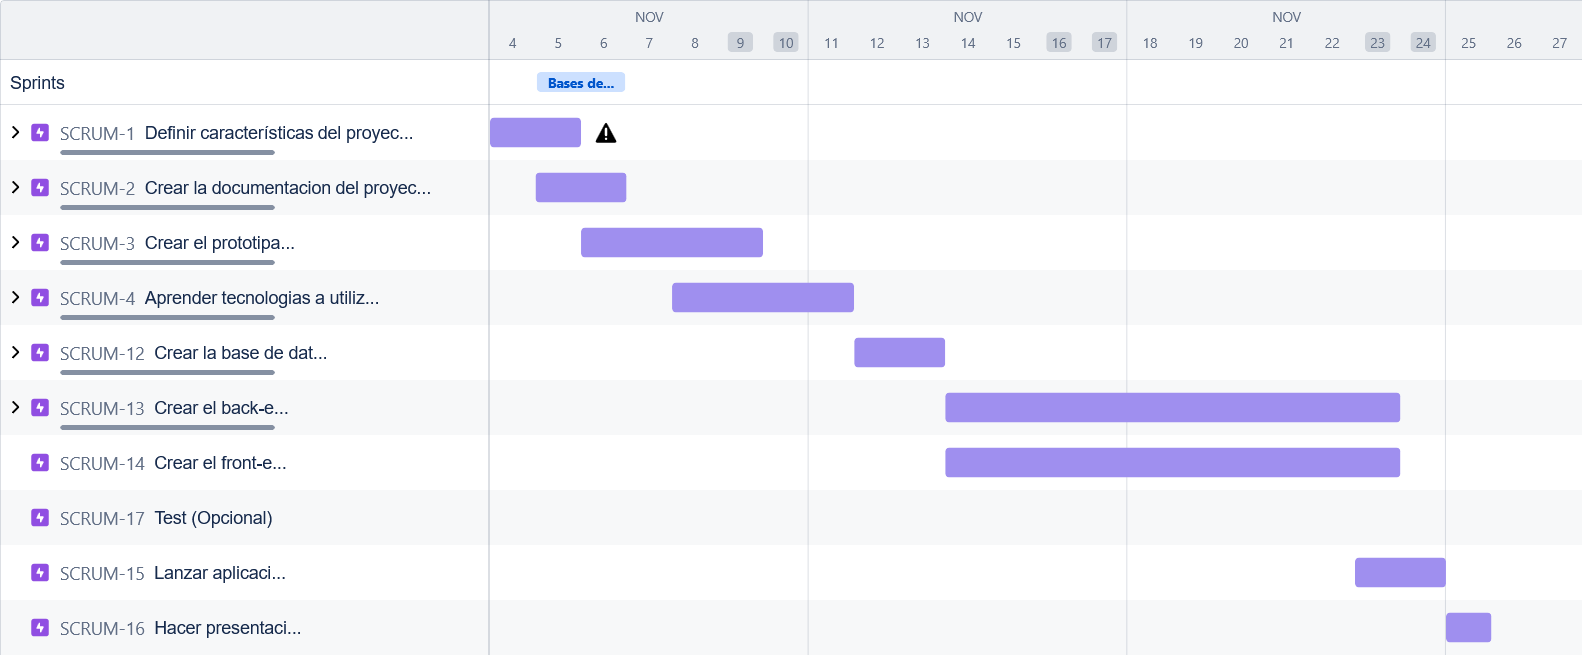
\includegraphics[width=0.9\linewidth]{./images/proyecto_final_ingr_2024-11-05_11.32am}
		\caption{Cronograma del Proyecto obtenido de JIRA}
	\end{figure}
	
	\pagebreak
	\section{Recursos y Roles}
	Recursos:
	\begin{itemize}
		\item 1 Líder de Proyecto
		\item 2 Desarrolladores
	\end{itemize}

	Roles: 
	\begin{itemize}
		\item Desarrollador Backend: Alejandro Macías Fonseca
		\item Desarrollador Backend: David Mata Guerra
		\item Desarrollador Frontend: Alexis Emilio Cárdenas Camacho
		\item Desarrollador Frontend: Gabriel Juárez Ramírez
	\end{itemize}
	
	\section{Control de Versiones}
	El control de versiones se llevó a cabo utilizando Git y GitHub. 
		\begin{center}
		
\includegraphics[width=0.3\linewidth]{./images/gitlogo.png}
		
\includegraphics[width=0.3\linewidth]{./images/github_logo.png}
	\end{center}


	Se crearon dos repositorios :
	\begin{itemize}
	  \item Backend: \href{https://github.com/dmataguerra/proyecto_final_ing_requerimientos_back}{Repositorio de GitHub}
		\href{https://github.com/dmataguerra/nestJS-prisma-test}{Repositorio de GitHub}
	  \item Frontend: \href{https://github.com/Alexiiis21/frontend.git}{Repositorio de GitHub}	
	\end{itemize}


	\section{Herramientas de Desarrollo}
	\begin{itemize}
		\item Documentación:
		\begin{itemize}
			\item LaTeX
		\end{itemize}
		\item Backend:
		\begin{itemize}
			\item Node.js
			\item Nest.js
			\item PostgreSQL
			\item Prisma
		\end{itemize}

		\item Frontend:
		\begin{itemize}
			\item React
			\item Next.js
			\item Shadcn
		\end{itemize}
	\end{itemize}
